% \iffalse meta-comment
%
% This is file `mcmthesis.dtx'.
%
% Copyright (C)
%     2010 -- 2015 by Zhaoli Wang
%     2014 -- 2015 by Liam Huang
% -----------------------------------
% This work may be distributed and/or modified under the
% conditions of the LaTeX Project Public License, either version 1.3
% of this license or (at your option) any later version.
% The latest version of this license is in
%   http://www.latex-project.org/lppl.txt
% and version 1.3 or later is part of all distributions of LaTeX
% version 2005/12/01 or later.
%
% This work has the LPPL maintenance status `maintained'.
%
% The Current Maintainer of this work is Liam Huang.
%
%<*internal>
\begingroup
  \def\temp{LaTeX2e}
\expandafter\endgroup\ifx\temp\fmtname\else
\csname fi\endcsname
%</internal>
%<*install>
\input docstrip.tex
\keepsilent
\preamble

-----------------------------------

This is a generated file.

Copyright (C)
    2010 -- 2015 by Zhaoli Wang
    2014 -- 2015 by Liam Huang

This work may be distributed and/or modified under the
conditions of the LaTeX Project Public License, either version 1.3
of this license or (at your option) any later version.
The latest version of this license is in
  http://www.latex-project.org/lppl.txt
and version 1.3 or later is part of all distributions of LaTeX
version 2005/12/01 or later.

This work has the LPPL maintenance status `maintained'.

The Current Maintainer of this work is Liam Huang.

\endpreamble
\postamble

This work consists of these files \jobname.dtx,
                                  figures/ and
                                  code/,
and the derived files             \jobname.cls,
                                  \jobname-demo.tex,
                                  README,
                                  LICENSE,
                                  \jobname.pdf and
                                  \jobname-demo.pdf.
\endpostamble

\generate{%
  \usedir{tex/latex/\jobname}%
  \file{\jobname.cls}{\from{\jobname.dtx}{class}}%
  \usedir{doc/latex/\jobname}%
  \file{\jobname-demo.tex}{\from{\jobname.dtx}{demo}}%
  \nopreamble\nopostamble
  \file{README.tex}{\from{\jobname.dtx}{readme}}%
  \file{LICENSE.tex}{\from{\jobname.dtx}{license}}%
}

\Msg{*************************************************************}
\Msg{*}
\Msg{* To finish the installation you have to}
\Msg{*}
\Msg{* produce the user manual run the file \jobname.dtx}
\Msg{* through XeLaTeX --shell-escape,}
\Msg{*}
\Msg{* produce the demo file run the file \jobname-demo.tex}
\Msg{* through XeLaTeX,}
\Msg{*}
\Msg{* move the following file into a directory searched}
\Msg{* \space\space by TeX:}
\Msg{*}
\Msg{* \space\space\jobname.cls to TEXMF/tex/latex/mcmthesis/,}
\Msg{* \space\space\jobname.dtx to TEXMF/source/latex/mcmthesis/,}
\Msg{* \space\space other files\space\space\space to
  TEXMF/doc/latex/mcmthesis/,}
\Msg{*}
\Msg{* and then run texhash.}
\Msg{*}
\Msg{* Happy TeXing!}
\Msg{*************************************************************}
\endbatchfile
%</install>
%<*internal>
\fi
%</internal>
%<*driver>
\ProvidesFile{mcmthesis.dtx}
  [2015/01/19 v5.1.0b Thesis Template For MCM/ICM]
\documentclass{ltxdoc}
\EnableCrossrefs
\CodelineIndex
\RecordChanges
\usepackage[UTF8, fntef, hyperref]{ctexcap}
\usepackage{hologo}
\usepackage{xcolor}
\usepackage{tabu}
\usepackage{longtable}
\usepackage{booktabs}
\usepackage{minted}
\usepackage{multirow}
\usepackage{amsmath}
\usemintedstyle{perldoc}
\AtBeginDocument{\hypersetup{hidelinks}}
\newcommand{\pkg}[1]{\textsf{#1}}
\newcommand{\env}[1]{\textsf{#1}}
\newcommand{\cntr}[1]{\textsf{#1}}
\newcommand{\XeLaTeX}{\hologo{XeLaTeX}}
\newcommand{\mem}[1]{\textcolor{blue}{\kaishu #1}}
\newcommand{\file}[1]{\textsf{#1}}
\newcommand{\path}[1]{\textsf{#1}}
\begin{document}
  \DocInput{\jobname.dtx}
\end{document}
%</driver>
% \fi
%
% \CheckSum{348}
%
% \CharacterTable
%  {Upper-case    \A\B\C\D\E\F\G\H\I\J\K\L\M\N\O\P\Q\R\S\T\U\V\W\X\Y\Z
%   Lower-case    \a\b\c\d\e\f\g\h\i\j\k\l\m\n\o\p\q\r\s\t\u\v\w\x\y\z
%   Digits        \0\1\2\3\4\5\6\7\8\9
%   Exclamation   \!     Double quote  \"     Hash (number) \#
%   Dollar        \$     Percent       \%     Ampersand     \&
%   Acute accent  \'     Left paren    \(     Right paren   \)
%   Asterisk      \*     Plus          \+     Comma         \,
%   Minus         \-     Point         \.     Solidus       \/
%   Colon         \:     Semicolon     \;     Less than     \<
%   Equals        \=     Greater than  \>     Question mark \?
%   Commercial at \@     Left bracket  \[     Backslash     \\
%   Right bracket \]     Circumflex    \^     Underscore    \_
%   Grave accent  \`     Left brace    \{     Vertical bar  \|
%   Right brace   \}     Tilde         \~}
%
% \changes{v1.0}{2013/05/12}{首次公开。}
%
% \GetFileInfo{\jobname.dtx}
%
% \DoNotIndex{\test}
%
% \title{\hypertarget{Chinese}{%
%   \textsf{\jobname} 文档类\thanks{这份文档是 \textsf{\jobname}~\fileversion
%   的说明文档,更新日期 \filedate。}}%
%   \makebox[0pt][l]{\hspace{1.5cm}\hyperlink{English}%
%     {\large$ \to $ English Version}}
% }
% \author{王昭礼 \\ \texttt{343083553@qq.com}\and 黄晨成 \\ \texttt{liamhuang0205+\jobname@gmail.com}}
% \date{\filedate}
%
% \maketitle
%
% \begin{abstract}
%   这份模板是美国大学生数学建模竞赛(MCM/ICM)的论文模板。模板遵循赛事官方的要求,设置了
%   页眉页脚、字体和控制页等内容。本文档对模板的使用做出了说明。
% \end{abstract}
%
% \section{模板介绍}
%
% 这份模板最早由王昭礼设计,并在往年参赛者的建议下不断改进。2014 年年初,黄晨成接手模板,
% 用 key-value 语法重构了文档选项,并修复了一些 bug。2015 年年初,黄晨成将模板使用
% \pkg{DocStrip} 的语法重构,并上传至 CTAN。
%
% \section{安装说明}
%
% \subsection{下载}
%
% 你可以到项目主页下载模板的最新版本,也可以关注 \href{http://latexstudio.net/}
% {\LaTeX Studio} 的相关更新,除去项目主页之外,不再维护任何镜像。
%
% \begin{quote}
%   \url{https://gitcafe.com/ChinaTeX/mcmthesis}
% \end{quote}
%
% 此外,文档类也已上传至 CTAN,你可以在 \TeX{} Live 等发行版的宏包管理器中下载。
%
% \subsection{安装}
%
% 我们以 \path{SOURCE} 代表你下载的源文件目录,在终端下执行以下命令。
% \iffalse
%<*internal>
% \fi
\begin{minted}{sh}
cd SOURCE
xelatex mcmthesis.ins
xelatex -shell-escape mcmthesis.dtx
xelatex -shell-escape mcmthesis.dtx
xelatex mcmthesis-demo.tex
xelatex mcmthesis-demo.tex
\end{minted}
% \iffalse
%</internal>
% \fi
%
% 你可以将生成的 \file{mcmthesis.cls} 拷贝至 \path{TEXMF/tex/latex/mcmthesis/}
% 目录,将 \file{mcmthesis.dtx} 和 \file{mcmthesis.ins} 拷贝至
% \path{TEXMF/source/latex/mcmthesis/},将 \file{mcmthesis.pdf}、
% \file{mcmthesis-demo.tex}、\file{mcmthesis-demo.pdf}、\file{figures/}
% 和 \file{code/} 拷贝至 \path{TEXMF/doc/latex/mcmthesis/},然后在终端
% 执行 \verb|texhash|;也可以将 \file{mcmthesis.cls} 放在当前目录直接使用。
%
% 生成的 \file{mcmthesis-demo.tex} 是一个示例文件,你可以参照这个文件来构建你的论文;
% 也可以直接修改这个文件。
%
% \section{使用说明}
% \subsection{依赖}
% \pkg{mcmthesis} 依赖于以下宏包,这些宏包在常见的 \TeX{} 发行版中都已包含,
% 在安装使用之前,请确认你的 \TeX{} 发行版中正确安装了这些宏包。
% \begin{longtabu}to 0.9\linewidth{*4{X[cm]}}
%   \toprule
%   \pkg{kvoptions} & \pkg{etoolbox} & \pkg{fancyhdr} & \pkg{fancybox} \\
%   \pkg{ifthen} & \pkg{lastpage} & \pkg{listings} & \pkg{appendix} \\
%   \pkg{amsmath} & \pkg{amssymb} & \pkg{amsfonts} & \pkg{amsbsy} \\
%   \pkg{bm} & \pkg{mathrsfs} & \pkg{latexsym} & \pkg{paralist} \\
%   \pkg{longtable} & \pkg{multirow} & \pkg{hhline} & \pkg{tabularx} \\
%   \pkg{ctex} & \pkg{xeCJK} & \pkg{CJK} & \pkg{xCJK2uni}\\
%   \pkg{tabu} & \pkg{minted} & \pkg{longtable} & \pkg{hologo}\\
%   \pkg{array} & \pkg{flafter} & \pkg{pifont} & \pkg{calc} \\
%   \pkg{colortbl} & \pkg{booktabs} & \pkg{geometry} & \pkg{fontenc}\\
%   \pkg{berasans} & \pkg{hyperref} & \pkg{ifpdf} & \pkg{ifxetex}\\
%   \pkg{graphicx} & \pkg{epstopdf} & \pkg{bmpsize} & \pkg{xcolor}\\
%   \pkg{longtable} & \pkg{tabu} & \pkg{hologo} & \pkg{palatino}\\
%   \pkg{mwe}\\
%   \bottomrule
% \end{longtabu}
% 如果你尚未安装这些宏包,可以启动你的 \TeX{} 发行版的宏包管理器
% 来安装;或者到 \url{http://www.ctan.org} 上搜索下载并安装。
%
% \subsection{选项}
% \pkg{mcmthesis} 有三个选项:
% \begin{description}
%   \item [tcn] 队伍控制号码,接受一个字符串作为值;输入的值将显示在控制页上和
%     每一页的页眉上;默认为 \texttt{0000}。
%   \item [sheet] 布尔值;为真时将输出控制页,否则不输出;默认为 \texttt{true}。
%   \item [abstract] 布尔值;为真时将在标题页输出摘要和关键词,否则不输出;默认值为
%     \texttt{true}。
% \end{description}
%
% 注意,模板提供了 \env{keywords} 环境。该环境的内容只在标题页的摘要下输出,不会在控制页
% 的摘要下输出。因此,若 \texttt{abstract = false},则不会输出关键词。
%
% \subsection{题号}
%
% 模板定义了 \cs{problem}\marg{题号} 命令,用以选择题号。
%
% \subsection{编译方式}
%
% 模板支持多种编译方式:
% \begin{itemize}
%   \item \XeLaTeX \textbf{这是推荐的方式};
%   \item pdf\LaTeX;
%   \item \LaTeX{} + DVIPDFMx。
% \end{itemize}
%
% \subsection{中文支持}
%
% 由于 MCM/ICM 要求以英文写作,所以模板没有内建的中文支持。如果你在文章中需要使用个别中文
% 字符,可以自行使用合适中文支持方式。
%
% 对于 \XeLaTeX{} 来说,可以使用 \pkg{xeCJK} 宏包。
% \iffalse
%<*internal>
% \fi
\begin{minted}{tex}
\usepackage{xeCJK}
\setCJKmainfont{SimSun}
\end{minted}
% \iffalse
%</internal>
% \fi
% 这里,Mac OS X 的用户可以使用 \texttt{STSong} 来代替 \texttt{SimSun};
% Linux 用户则可以使用 \texttt{FandolSong}。
%
% 对于 pdf\LaTeX{} 和 \LaTeX{} + DVIPDFMx 来说,可以使用 \pkg{zhmCJK} 宏包。
% \iffalse
%<*internal>
% \fi
\begin{minted}{tex}
\usepackage{zhmCJK}
\setCJKmainfont{SimSun.ttc}
\end{minted}
% \iffalse
%</internal>
% \fi
% 对 Mac OS X 和 Linux 的说明同上。
%
%
%
% \title{\hypertarget{English}{%
%   The \textsf{\jobname} class\thanks{This Document
%   corresponds to \textsf{\jobname}~\fileversion, dated \filedate.}}%
%   \makebox[0pt][l]{\hspace{1.5cm}\hyperlink{Chinese}{\large$ \to $ 中文版}}
% }
% \author{Zhaoli Wang \\ \texttt{\texttt{343083553@qq.com}}\and Liam Huang \\ \texttt{liamhuang0205+\jobname@gmail.com}}
% \date{\filedate}
%
% \maketitle
%
% \begin{abstract}
%   This template is designed for MCM/ICM. The template configured fonts,
%   header and footer and control sheet style, accroding to the requirements
%   of COMAP. This document desicribes the template.
% \end{abstract}
%
% \section{Introduction}
%
% This template was designed by Zhaoli Wang first, and was improved by him
% following the suggestions from contest takers. In the beginning of the year
% 2014, Liam Huang redesigned it, by using key-value syntax, and fixed known
% bugs. Liam reimplemented it at the begining of the year 2015,
% by \pkg{DocStrip}, and uploaded it to CTAN.
%
% \section{Installation Guide}
%
% \subsection{Download}
%
% You could find the latest version of this template at the project homepage,
% as well as the website \href{http://latexstudio.net/}{\LaTeX Studio}. We will
% not maintain any other mirror.
%
% \begin{quote}
%   \url{https://github.com/LiamHuang0205/mcmthesis}
% \end{quote}
%
% Moreover, this template had been uploaded to CTAN, so that it could
% be managed by the package manager of your distribution, such as \TeX\ Live.
%
% \subsection{Installation}
%
% We denote \path{SOURCE} as the folder, who contains the file you've
% just downloaded. Execute these command in the terminal.
% \iffalse
%<*internal>
% \fi
\begin{minted}{sh}
cd SOURCE
xelatex mcmthesis.ins
xelatex -shell-escape mcmthesis.dtx
xelatex -shell-escape mcmthesis.dtx
xelatex mcmthesis-demo.tex
xelatex mcmthesis-demo.tex
\end{minted}
% \iffalse
%</internal>
% \fi
%
% To finish the installation, you could copy \file{mcmthesis.cls} to
% \path{TEXMF/tex/latex/mcmthesis/}, copy \file{mcmthesis.dtx}
% and \file{mcmthesis.ins} to \path{TEXMF/source/latex/mcmthesis/},
% copy \file{mcmthesis.pdf}, \file{mcmthesis-demo.tex},
% \file{mcmthesis-demo.pdf}, \file{figures/} and \file{code/} to
% \path{TEXMF/doc/latex/mcmthesis/}, and then run \verb|texhash| in your
% terminal; you could also put \file{mcmthesis.cls} in the same folder of
% the master file.
%
% \file{mcmthesis-demo.tex} is a generated demo file, you could write the
% manuscript of you paper by mimicing this file; you may also modify this
% file to build your paper.
%
% \section{Usage}
% \subsection{Dependence}
% The \pkg{mcmthesis} class depends on the following pakcages.
% These packages has been installed in common \TeX{} distribution.
% Before installation, please make sure that you have installed these
% packages correctly.
% \begin{longtabu}to 0.9\linewidth{*4{X[cm]}}
%   \toprule
%   \pkg{kvoptions} & \pkg{etoolbox} & \pkg{fancyhdr} & \pkg{fancybox} \\
%   \pkg{ifthen} & \pkg{lastpage} & \pkg{listings} & \pkg{appendix} \\
%   \pkg{amsmath} & \pkg{amssymb} & \pkg{amsfonts} & \pkg{amsbsy} \\
%   \pkg{bm} & \pkg{mathrsfs} & \pkg{latexsym} & \pkg{paralist} \\
%   \pkg{longtable} & \pkg{multirow} & \pkg{hhline} & \pkg{tabularx} \\
%   \pkg{ctex} & \pkg{xeCJK} & \pkg{CJK} & \pkg{xCJK2uni}\\
%   \pkg{tabu} & \pkg{minted} & \pkg{longtable} & \pkg{hologo}\\
%   \pkg{array} & \pkg{flafter} & \pkg{pifont} & \pkg{calc} \\
%   \pkg{colortbl} & \pkg{booktabs} & \pkg{geometry} & \pkg{fontenc}\\
%   \pkg{berasans} & \pkg{hyperref} & \pkg{ifpdf} & \pkg{ifxetex}\\
%   \pkg{graphicx} & \pkg{epstopdf} & \pkg{bmpsize} & \pkg{xcolor}\\
%   \pkg{longtable} & \pkg{tabu} & \pkg{hologo} & \pkg{palatino}\\
%   \pkg{mwe}\\
%   \bottomrule
% \end{longtabu}
% If you haven't install these packages, you could execute the package
% manager of your distribution and install them; you could also download
% them from \url{http://www.ctan.org}.
%
% \subsection{Options}
% \pkg{mcmthesis} has three options:
% \begin{description}
%   \item [tcn] The team control number, recieves a string as value;
%     this value will be displayed on control sheet and every page's header.
%     The default value is \texttt{0000}.
%   \item [sheet] Bool, true to print the control sheet, default
%     is \texttt{true}.
%   \item [abstract] Bool, true to print the abstract on the titlepage,
%     default is \texttt{true}.
% \end{description}
%
% Note that the template provides the \env{keywords} environment, whose
% contents will only be displayed after the abstract on titlepage, and
% will not be displayed on the control sheet. Thus, if one set
% \texttt{abstract = false}, keywords will not be printed.
%
% \subsection{Question}
%
% The template defines \cs{problem}\marg{question} to choose the question.
%
% \subsection{Compilation Workflow}
%
% The template supports various kinds of compilation workflow:
% \begin{itemize}
%   \item \XeLaTeX\ (\textbf{recommend});
%   \item pdf\LaTeX;
%   \item \LaTeX{} + DVIPDFMx。
% \end{itemize}
%
%
% \StopEventually{}
% \section{The Implementation}
% \subsection{Basic Information}
%    \begin{macrocode}
%<*class>
\NeedsTeXFormat{LaTeX2e}[1999/12/01]
\ProvidesClass{mcmthesis}
  [2015/01/19 v5.1.0b Thesis Template For MCM/ICM]
\typeout{Thesis Template For MCM/ICM}
\def\MCMversion{v5.1.0b}
%    \end{macrocode}
% \subsection{Options}
%
% Loading \pkg{kvoptions} and \pkg{etoolbox} to handle key-value options.
%    \begin{macrocode}
\RequirePackage{kvoptions}
\RequirePackage{etoolbox}
\SetupKeyvalOptions{family=MCM, prefix=MCM@opt@, setkeys=\kvsetkeys}
\newcommand{\skv}[1]{\kvsetkeys{MCM}{#1}}
%    \end{macrocode}
%
% Declaring options.
%    \begin{macrocode}
\DeclareBoolOption[true]{sheet}
\DeclareComplementaryOption{nosheet}{sheet}
\DeclareBoolOption[true]{abstract}
\DeclareComplementaryOption{noabstract}{abstract}
\DeclareStringOption[0000]{tcn}[0000]
\DeclareDefaultOption{\relax}
%    \end{macrocode}
% Processing options.
%    \begin{macrocode}
\ProcessKeyvalOptions*\relax
%    \end{macrocode}
%
% Loading document class.
%    \begin{macrocode}
\LoadClass[a4paper, 11pt]{article}
%    \end{macrocode}
%
% User interface.
%    \begin{macrocode}
\newcommand{\control}{\MCM@opt@tcn}
\newcommand{\team}{Team \#\ \MCM@opt@tcn}
%    \end{macrocode}
% \subsection{Loading Packages}
%    \begin{macrocode}
\RequirePackage{fancyhdr, fancybox}
\RequirePackage{ifthen}
\RequirePackage{lastpage}
\RequirePackage{listings}
\RequirePackage[toc, page, title, titletoc, header]{appendix}
\RequirePackage{paralist}
\RequirePackage{amsthm, amsfonts}
\RequirePackage{amsmath, bm}
\RequirePackage{amssymb, mathrsfs}
\RequirePackage{latexsym}
\RequirePackage{longtable, multirow, hhline, tabularx, array}
\RequirePackage{flafter}
\RequirePackage{pifont, calc}
\RequirePackage{colortbl, booktabs}
\RequirePackage{geometry}
\RequirePackage[T1]{fontenc}
\RequirePackage[scaled]{berasans}
\RequirePackage{hyperref}
\RequirePackage{ifpdf, ifxetex}
%    \end{macrocode}
%
% Loading \pkg{graphicx} and its relations after checking drivers.
%    \begin{macrocode}
\ifpdf
  \RequirePackage{graphicx}
  \RequirePackage{epstopdf}
\else
  \ifxetex
    \RequirePackage{graphicx}
  \else
    \RequirePackage[dvipdfmx]{graphicx}
    \RequirePackage{bmpsize}
  \fi
\fi
\RequirePackage{xcolor}
%    \end{macrocode}
% \subsection{\pkg{hyperref} Settings}
%    \begin{macrocode}
\ifpdf
  \hypersetup{hidelinks}
\else
  \ifxetex
    \hypersetup{hidelinks}
  \else
    \hypersetup{dvipdfm, hidelinks}
  \fi
\fi
%    \end{macrocode}
% \subsection{Page Layout}
% Setting paper size and margin sep.
%    \begin{macrocode}
\geometry{a4paper, margin = 1.2in}
%    \end{macrocode}
%
% Making the footer and header.
%    \begin{macrocode}
\pagestyle{fancy}
\fancyhf{}
\lhead{\small \team}
\rhead{\small Page \thepage\ of \pageref{LastPage}}
%    \end{macrocode}
%
% Setting \cs{parskip}.
%    \begin{macrocode}
\setlength\parskip{.5\baselineskip}
%    \end{macrocode}
% \subsection{Redefining TOC}
%    \begin{macrocode}
\renewcommand\tableofcontents{%
    \centerline{\normalfont\Large\bfseries\contentsname
        \@mkboth{%
           \MakeUppercase\contentsname}{\MakeUppercase\contentsname}}%
    \vskip 5ex%
    \@starttoc{toc}%
    }
%    \end{macrocode}
% \subsection{Mastering Floats, Figures and Tables}
% Setting counters. Here \cntr{totalnumber} is the maximum number of
% floats on a text page, \cntr{topnumber} is the maximum number of
% floats at top of a text page and \cntr{bottomnumber} is the maximum
% number of floats at bottom of a text page. Obviously, we have
% $ \text{\cntr{totalnumber}} = \text{\cntr{topnumber}} +
% \text{\cntr{bottomnumber}} $.
%    \begin{macrocode}
\setcounter{totalnumber}{4}
\setcounter{topnumber}{2}
\setcounter{bottomnumber}{2}
%    \end{macrocode}
%
% Setting float fractions.
%    \begin{macrocode}
\renewcommand{\textfraction}{0.15}
\renewcommand{\topfraction}{0.85}
\renewcommand{\bottomfraction}{0.65}
\renewcommand{\floatpagefraction}{0.60}
%    \end{macrocode}
%
% Setting caption names.
%    \begin{macrocode}
\renewcommand{\figurename}{Figure}
\renewcommand{\tablename}{Table}
%    \end{macrocode}
%
% Setting graphic paths.
%    \begin{macrocode}
\graphicspath{{./}{./img/}{./fig/}{./image/}{./figure/}{./picture/}
            {./imgs/}{./figs/}{./images/}{./figures/}{./pictures/}}
%    \end{macrocode}
% \subsection{Designing Sheets and their Relations}
% Redefining \cs{@maketitle}, which is executed by \cs{maketitle}.
% \cs{@maketitle} will check if the control sheet and abstract (on title
% page) should be printed.
%
% Note that the keywords will only be printed on the titlepage.
%    \begin{macrocode}
\def\@maketitle{%
  \ifMCM@opt@sheet%
  \makesheet%
  \fi
  \newpage
  \null
  \vskip 2em%
  \begin{center}%
  \let \footnote \thanks
    {\LARGE \@title \par}%
    \vskip 1.5em%
    {\large
      \lineskip .5em%
      \begin{tabular}[t]{c}%
        \@author
      \end{tabular}\par}%
    \vskip 1em%
    {\large \@date}%
  \end{center}%
  \par
  \vskip 1.5em%
  \ifMCM@opt@abstract%
  \make@abstract%
  \fi%
}
%    \end{macrocode}
%
% Making the \env{abstract} environment.
%    \begin{macrocode}
\def\keywordsname{{\bfseries Keywords:}}
\def\@abstract{}%
\newbox\@abstract%
\setbox\@abstract\hbox{}%
\long\def\abstract{\bgroup\global\setbox\@abstract%
  \vbox\bgroup\hsize\textwidth\leftskip1cm\rightskip1cm}%
\def\endabstract{\egroup\egroup}
\newbox\@keywords
\setbox\@keywords\hbox{}
\def\keywords{\bgroup\global\setbox\@keywords\vbox\bgroup\noindent\leftskip0cm}
\def\endkeywords{\egroup\egroup}%
\def\make@abstract{%
\par%
\centerline{\bfseries\abstractname}\vskip5pt\par%
\noindent\usebox\@abstract\par%
\noindent\hskip1cm\keywordsname\ \usebox\@keywords%
\vskip10pt%
}
%    \end{macrocode}
%
% Defining the \cs{makesheet}.
%    \begin{macrocode}
\newcommand{\@problem}[1]{}
\newcommand{\problem}[1]{\gdef\@problem{#1}}
\def\makesheet{%
  \null%
  \vskip 3em%
  \begingroup\fontfamily{fvs}\fontseries{m}\selectfont%
  \thispagestyle{empty}%
  \noindent\begin{tabularx}{0.3\textwidth}{lX}%
  \multicolumn{2}{l}{For office use only}\\
    T1&\rule{3cm}{0.5pt}\\
    T2&\rule{3cm}{0.5pt}\\
    T3&\rule{3cm}{0.5pt}\\
    T4&\rule{3cm}{0.5pt}\\
    \end{tabularx}\hspace{\fill}
    \begin{minipage}{0.33\textwidth}
    \centering
    Team Control Number\\[10pt]
    {\fontsize{38pt}{25pt}\selectfont  \textbf{\MCM@opt@tcn} }%
      \normalsize\\[10pt]
    Problem Chosen\\[10pt]
    {\fontsize{20pt}{\baselineskip}\selectfont \textbf{\@problem}}\normalsize\\
    \end{minipage}\hspace{\fill}
    \begin{tabularx}{0.28\textwidth}{lX}%
    \multicolumn{2}{l}{For office use only}\\
    F1&\rule{3cm}{0.5pt}\\
    F2&\rule{3cm}{0.5pt}\\
    F3&\rule{3cm}{0.5pt}\\
    F4&\rule{3cm}{0.5pt}\\
    \end{tabularx}\par
\noindent\rule{\textwidth}{0.5pt}\par
\begin{center}
  \textbf{\the\year\ Mathematical Contest in Modeling (MCM) Summary Sheet}\\
(Attach a copy of this page to each copy of your solution paper.)
\end{center}
\par%
\vskip 1.5em%
\centerline{\large\bfseries\abstractname}
\noindent\usebox\@abstract%
\endgroup}
%    \end{macrocode}
% \subsection{Mathematics}
% Theorems.
%    \begin{macrocode}
\newtheorem{Theorem}{Theorem}[section]
\newtheorem{Lemma}[Theorem]{Lemma}
\newtheorem{Corollary}[Theorem]{Corollary}
\newtheorem{Proposition}[Theorem]{Proposition}
\newtheorem{Definition}[Theorem]{Definition}
\newtheorem{Example}[Theorem]{Example}
%    \end{macrocode}
%
% Other definitions.
%    \begin{macrocode}
\providecommand{\dif}{\mathop{}\!\mathrm{d}}
\providecommand{\me}{\mathrm{e}}
\providecommand{\mi}{\mathrm{i}}
%    \end{macrocode}
% \subsection{Listing Settings}
%    \begin{macrocode}
\definecolor{grey}{rgb}{0.8,0.8,0.8}
\definecolor{darkgreen}{rgb}{0,0.3,0}
\definecolor{darkblue}{rgb}{0,0,0.3}
\def\lstbasicfont{\fontfamily{pcr}\selectfont\footnotesize}
\lstset{%
% indexing
   % numbers=left,
   % numberstyle=\small,%
% character display
    showstringspaces=false,
    showspaces=false,%
    tabsize=4,%
% style
    frame=lines,%
    basicstyle={\footnotesize\lstbasicfont},%
    keywordstyle=\color{darkblue}\bfseries,%
    identifierstyle=,%
    commentstyle=\color{darkgreen},%\itshape,%
    stringstyle=\color{black}%
}
\lstloadlanguages{C,C++,Java,Matlab,Mathematica}
%    \end{macrocode}
%    \begin{macrocode}
%</class>
%<class>\endinput
%    \end{macrocode}
% \iffalse
%<*demo>
%!TEX program = xelatex
\documentclass[tcn = 0000, sheet = true, abstract = true]{mcmthesis}
\problem{A}
\usepackage{palatino}
\usepackage{mwe}
\title{The \LaTeX{} Template for MCM Version 5.1.0b}
\author{\small \href{http://www.latexstudio.net/}
  {
\includegraphics[width=7cm]{mcmthesis-logo}}}
\date{\today}
\begin{document}
\begin{abstract}
\lipsum[1]
\begin{keywords}
keyword1; keyword2
\end{keywords}
\end{abstract}
\maketitle
\newpage
% Generate the Table of Contents, if it's needed.
% \tableofcontents
% \newpage
\section{Introduction}

\lipsum[2]
\begin{itemize}
\item minimizes the discomfort to the hands, or
\item maximizes the outgoing velocity of the ball.
\end{itemize}
We focus exclusively on the second definition.

\begin{itemize}
\item the initial velocity and rotation of the ball,
\item the initial velocity and rotation of the bat,
\item the relative position and orientation of the bat and ball, and
\item the force over time that the hitter hands applies on the handle.
\end{itemize}
\lipsum[3]
\begin{itemize}
\item the angular velocity of the bat,
\item the velocity of the ball, and
\item the position of impact along the bat.
\end{itemize}
\lipsum[4]
\emph{center of percussion} [Brody 1986], \lipsum[5]

\begin{Theorem} \label{thm:latex}
\LaTeX
\end{Theorem}
\begin{Lemma} \label{thm:tex}
\TeX .
\end{Lemma}
\begin{proof}
The proof of theorem.
\end{proof}

\subsection{Other Assumptions}
\lipsum[6]
\begin{itemize}
\item
\item
\item
\item
\end{itemize}

\lipsum[7]

\section{Analysis of the Problem}
\begin{figure}[h]
\small
\centering
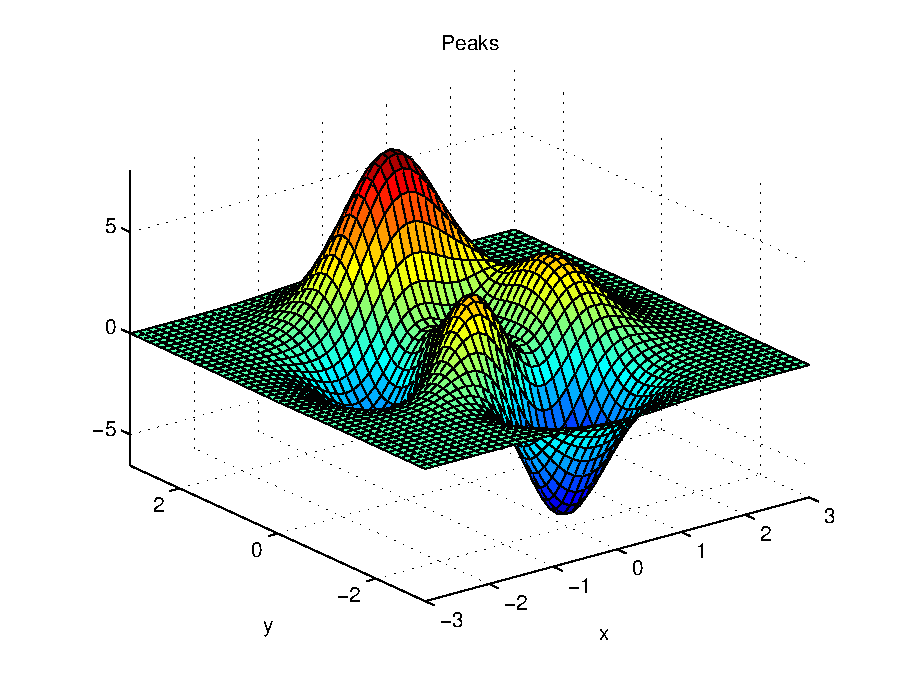
\includegraphics[width=12cm]{mcmthesis-aaa.eps}
\caption{aa} \label{fig:aa}
\end{figure}

\lipsum[8] \eqref{aa}
\begin{equation}
a^2 \label{aa}
\end{equation}


\[
  \begin{pmatrix}{*{20}c}
  {a_{11} } & {a_{12} } & {a_{13} }  \\
  {a_{21} } & {a_{22} } & {a_{23} }  \\
  {a_{31} } & {a_{32} } & {a_{33} }  \\
  \end{pmatrix}
  = \frac{{Opposite}}{{Hypotenuse}}\cos ^{ - 1} \theta \arcsin \theta
\]
\lipsum[9]

\[
  p_{j}=\begin{cases} 0,&\text{if $j$ is odd}\\
  r!\,(-1)^{j/2},&\text{if $j$ is even}
  \end{cases}
\]

\lipsum[10]

\[
  \arcsin \theta  =
  \mathop{{\int\!\!\!\!\!\int\!\!\!\!\!\int}\mkern-31.2mu
  \bigodot}\limits_\varphi
  {\mathop {\lim }\limits_{x \to \infty } \frac{{n!}}{{r!\left( {n - r}
  \right)!}}} \eqno (1)
\]

\section{Calculating and Simplifying the Model  }
\lipsum[11]

\section{The Model Results}
\lipsum[6]

\section{Validating the Model}
\lipsum[9]

\section{Conclusions}
\lipsum[6]

\section{A Summary}
\lipsum[6]

\section{Evaluate of the Mode}

\section{Strengths and weaknesses}
\lipsum[12]

\subsection{Strengths}
\begin{itemize}
\item \textbf{Applies widely}\\
This  system can be used for many types of airplanes, and it also
solves the interference during  the procedure of the boarding
airplane,as described above we can get to the  optimization
boarding time.We also know that all the service is automate.
\item \textbf{Improve the quality of the airport service}\\
Balancing the cost of the cost and the benefit, it will bring in
more convenient  for airport and passengers.It also saves many
human resources for the airline. \item \textbf{}
\end{itemize}

\begin{thebibliography}{99}
%\addcontentsline{toc}{section}{References}
\bibitem{1} D.~E. KNUTH   The \TeX{}book  the American
Mathematical Society and Addison-Wesley
Publishing Company , 1984-1986.
\bibitem{2}Lamport, Leslie,  \LaTeX{}: `` A Document Preparation System '',
Addison-Wesley Publishing Company, 1986.
\bibitem{3}\url{http://www.latexstudio.net/}
\bibitem{4}\url{http://www.chinatex.org/}
\end{thebibliography}

\begin{appendices}

\section{First appendix}

\lipsum[13]

Here are simulation programmes we used in our model as follow.\\

\textbf{\textcolor[rgb]{0.98,0.00,0.00}{Input matlab source:}}
\lstinputlisting[language=Matlab]{./code/mcmthesis-matlab1.m}

\section{Second appendix}

some more text \textcolor[rgb]{0.98,0.00,0.00}{\textbf{Input C++ source:}}
\lstinputlisting[language=C++]{./code/mcmthesis-sudoku.cpp}

\end{appendices}
\end{document}

%</demo>
%<*readme>
# The `mcmthesis` Class

This class is designed for the MCM/ICM.

This work is released under the [LaTeX Project Public
License](http://www.latex-project.org/lppl.txt), v1.3c or later.

## Installation

This work consists of the file mcmthesis.dtx,
                               figures/, and
                               code/,
and the derived files          mcmthesis.cls,
                               mcmthesis-demo.tex,
                               README,
                               LICENSE,
                               mcmthesis.pdf and
                               mcmthesis-demo.pdf.

To install this class, you should
    move `mcmthesis.cls` to `TEXMF/tex/latex/mcmthesis/`,
    move `mcmthesis.dtx` to `TEXMF/source/latex/mcmthesis/`,
    move other files     to `TEXMF/doc/latex/mcmthesis/` and then
    run `texhash`.

## Author

[Zhaoli Wang][zhaoli]

Email: 343083553@qq.com

[Liam Huang][liam-ctan]

Email: liamhuang0205+mcmthesis@gmail.com

## Project Page

If you are interested in the process of development you may observe

<https://github.com/LiamHuang0205/mcmthesis>

[zhaoli]: http://www.latexstudio.net/
[liam-ctan]: http://www.ctan.org/author/huang-l
%</readme>
%<*license>
Released under the [LaTeX Project Public License]
(http://www.latex-project.org/lppl.txt), v1.3c or later.

The package has status 'maintained': the current maintainer is
[Liam Huang](liamhuang0205+mcmthesis@gmail.com).
%</license>
% \fi
% \Finale
\endinput
%%
%% This work consists of the file  mcmthesis.dtx, mcmthesis.ins,
%%                                 figures/, and code/,
%% and the derived files           mcmthesis.cls,
%%                                 mcmthesis-demo.tex,
%%                                 README,
%%                                 LICENSE,
%%                                 mcmthesis.pdf and
%%                                 mcmthesis-demo.pdf.
%%
%% End of file `mcmthesis.dtx'.
